\chapter{Data Processing Examples}
\label{ch:examples}

\definecolor{lgray}{gray}{0.95}

This chapter showcases a variety of results that are possible when
processing different data sets with the Stereo Pipeline. It is also a
shortened guide that shows the commands and recommended settings to
process specific mission data. We hope that this serves as cookbook
for strategies that will get you started in processing your own data.

\section{Guidelines for Selecting Stereo Pairs}

When choosing image pairs to process, images that are taken with
similar viewing angles, lighting conditions, and significant surface
coverage overlap are best suited for creating terrain
models. Depending on the characteristics of the mission data set and
the individual images, the degree of acceptable variation will
differ. Significant differences between image characteristics
increases the likelihood of stereo matching error and artifacts, and
these errors will propagate through to the resulting data products.

Although images do not need to be map projected before running the
\texttt{stereo} program, we recommend that you do run {\tt cam2map}
(or \texttt{cam2map4stereo.py})
beforehand, especially for image pairs that contain large topographic
variation (and therefore large disparity differences across the
scene, e.g. Valles Marineris).  Map projection is especially necessary
when processing \ac{HiRISE} images. This removes the large disparity
differences between \ac{HiRISE} images and leaves only the small
detail for the Stereo Pipeline to compute. Remember that \ac{ISIS}
can work backwards through a map-projection when applying the camera
model, so the geometric integrity of your images will not be sacrificed
if you map project first.

Excessively noisy images will not correlate well, so images should be
photometrically calibrated in whatever fashion suits your purposes. If
there are photometric problems with the images, those photometric
defects can be misinterpreted as topography.

Remember, in order for \texttt{stereo} to process stereo pairs in
\ac{ISIS} cube format, the images must have had SPICE data associated
by running ISIS's \texttt{spiceinit} program run on them first.

\subsection{Combatting long run times}

The factor that predominantly determines running time in the Stereo
Pipeline is the size of the search space considered by the correlation
algorithm.  These are set in the \texttt{stereo.default} file using
the \texttt{corr-search} parameter.  If you comment that parameter out
(either by putting a `\texttt{\#}' at the beginning of their line or
deleting them from your \texttt{stereo.default} file), the Stereo
Pipeline will try to automatically determine the search range for you,
but this does not always work perfectly.  A spurious bad match can
lead the pipeline to select a search range that is far too large, and
performance will suffer as a result.  If you know (or can estimate)
the range of horizontal and vertical offsets you expect to see between
the two images, then you may want to try setting the search range
yourself in your \texttt{stereo.default} using the aforementioned
parameters.

More generally, here are three strategies that tend to keep the
search range small and run-times low:

\begin{enumerate}
\item You can crop your stereo pair (using the ISIS \texttt{crop}
command) to a small region of interest within a large stereo pair.
ISIS and the Stereo Pipeline will keep track of these crop parameters
automatically and take them into account when applying the camera
model during triangulation.  You may want to work with a cropped
pair when you first start working with a new data set.  Run times
will be much lower (minutes instead of days), and you can quickly
tune parameters in the \texttt{stereo.default} file before scaling
up to the full image.

\item The ISIS \texttt{reduce} command can be used to subsample the
image pair.  In this case, you are trading resolution for speed,
so this probably only makes sense for debugging or ``previewing'' 3D
terrain. That said, subsampling will tend to increase the signal
to noise ratio, so it may also be helpful for pulling 3D terrain
out of noisy, low quality images.

These options of croping or reducing the resolution of the source
imagery are only easily achieved with ISIS sessions. Pinhole and
Digital Globe sessions will be required to manually edit their camera
models in the event that you have edited the source imagery. This is
a unique problem for each camera model and thus will not be discussed
here.

\item You can map project the images (using the ISIS \texttt{cam2map}
command or the \texttt{cam2map4stereo.py} program provided with the
Stereo Pipeline).  If you project both images into the same map
projection and same pixel scale, then they will be aligned modulo
uncertainty in spacecraft telemetry (typically 10-100's of meters
of error when the image is projected onto the ground).  By default
\texttt{cam2map} will also project the image onto the local elevation
model (MOLA or LOLA), which removes the stereo disparity in the
images that is due to coarse topography.  The resulting image pair
has only small position offsets and fine 3D detail left to discover,
so the search range can be kept very small and run times can be
improved.  Again, ISIS and the Stereo Pipeline will keep track of
how these map projections affect the camera model, and take them
into account when building up the 3D mesh via triangulation.  If
you use \texttt{cam2map}, be sure that your \texttt{stereo.default}'s
\texttt{alignment-method} is set to NONE.  Note also that the
\texttt{-\/-lat} and \texttt{-\/-lon} arguments to
\texttt{cam2map4stereo.py} can be used to crop your stereo images,
and the \texttt{-\/-resolution} argument can be used to subsample
them.
\end{enumerate}

If you are working with very large images, we highly recommend
cropping or subsampling and working with smaller sized images while
you fine-tune the parameters in the \texttt{stereo.default} file,
and once you get satisfactory results to apply those parameters to
the full images.

%% \subsection{Comparing Examples to your System}

%% Since our first release we re-performed some of these examples and
%% recorded their processing time so you the user can judge how long it
%% will take you. Our examples were processed on our server called
%% `Lunokhod 2'. This server is a Dell PowerEdge Rack 900 purchased in
%% late 2009. Below are its specifications:

%% \begin{center}
%% \begin{tabular}{ l | l }
%% CPU & Dual E7420 Xeon at 2.13 GHz \emph{(16 logical cores)} \\ \hline
%% FSB & 1066 MHz \\ \hline
%% L2 Cache & 8 MB \\ \hline
%% Memory & 64 GB @ 667 MHz (mis-matched?) \\ \hline
%% Storage & Local RAID5 \\ \hline
%% OS & Red Hat Enterprise Linux 5.5 \\ \hline
%% BogoMIPS & 4256 \\ \hline
%% Color & Dell Graphite \\
%% \end{tabular}
%% \end{center}

%% The times recorded are listed in wall hours and CPU hours. Wall-hours
%% are how long it took the job to complete from the user's
%% perspective. CPU-hours are how much processing time it took to
%% complete. If the job took 30 wall-minutes on a 2 core system, it spent
%% 30 minutes in CPU 1 and CPU 2. Thus, the total CPU-hours would be
%% 1. This example, though correct, is not what always happens in the
%% real world. Inefficiency with managing multiple threads or the
%% complete lack of multithreaded code will bring wall hours up to CPU
%% hours. Your required CPU hours will vary based on CPU
%% architecture. Estimating your required CPU hours for your system can
%% be done by scaling with the BogoMIPS measurements. This can be read
%% from Linux systems with the command: \texttt{cat /proc/cpuinfo}

\section{Mars Reconnaissance Orbiter HiRISE}

\ac{HiRISE} is one of the most challenging cameras to use when making 3D
models because \ac{HiRISE} exposures can be several gigabytes each. Working
with this data requires patience as it will take time.

One important fact to know about HiRISE is that it is composed of
multiple linear CCDs that are arranged side by side with some vertical
offsets. These offsets mean that the CCDs will view some of the same
terrain but at a slightly different time and a slightly different
angle. Mosaicking the CCDs together to a single image is not a simple
process and involves living with some imperfections.

One cannot simply use the \ac{HiRISE} RDR products, as they do not
have the required geometric stability.  Instead, the \ac{HiRISE}
EDR products must be assembled using \ac{ISIS} \texttt{noproj}.
The USGS distributes a script in use by the \ac{HiRISE} team that
works forward from the team-produced `balance' cubes, which provides
a de-jittered, noproj'ed mosaic of a single observation, which is
perfectly suitable for use by the Stereo Pipeline (this script was
originally engineered to provide input for SOCET SET).  However,
the `balance' cubes are not available to the general public, and
so we include a program (\texttt{hiedr2mosaic.py}, written in
\href{http://www.python.org}{Python}) that will take \ac{PDS}
available \ac{HiRISE} EDR products and walk through the processing
steps required to provide good input images for \texttt{stereo}.

The program takes all the red CCDs and projects them using the \ac{ISIS}
{\tt noproj} command into the perspective of the RED5 CCD. From there,
{\tt hijitreg} is performed to work out the relative offsets between
CCDs. Finally the CCDs are mosaicked together using the average
offset listed from {\tt hijitreg} using the {\tt handmos} command.
Below is an outline of the processing.

\begin{verbatim}
    hi2isis           # Import HiRISE IMG to Isis
    hical             # Calibrate
    histitch          # Assemble whole-CCD images from the channels
    spiceinit
    spicefit          # For good measure
    noproj            # Project all images into perspective of RED5
    hijitreg          # Work out alignment between CCDs
    handmos           # Mosaic to single file
\end{verbatim}

To use our script, first go to the directory where you have downloaded
the HiRISE's RED EDR \texttt{IMG} files. You can run the 
\texttt{hiedr2mosaic.py} program without any arguments to view a short
help statement, with the \texttt{-h} option to view a longer help statement,
or just run the program on the EDR files like so:

\begin{verbatim}
    hiedr2mosaic.py *.IMG
\end{verbatim}

If you have more than one observation's worth of EDRs in that
directory, then limit the program to just one observation's EDRs
at a time, e.g. \texttt{hiedr2mosaic.py PSP\_001513\_1655*IMG}.  If you
run into problems, try using the \texttt{-k} option to retain all of 
the intermediary image files to help track down the issue.  The
\texttt{hiedr2mosaic.py} program will create a single mosaic file 
with the extension \texttt{.mos\_hijitreged.norm.cub}.  Be warned that
the operations carried out by \texttt{hiedr2mosaic.py} can take many 
hours to complete on the very large HiRISE images.

Finally we recommend map projecting the product and normalizing both
images in the stereo pair using the same dynamic range. Notice that we
map project the second image using the same map settings and crop of
the first image. This means the images will share the same origin and
the {\tt stereo.default} search range can be centered around zero.

\begin{verbatim}
  ISIS 3> cam2map4stereo.py first.mos_hijitreged.norm.cub second.mos_hijitreged.norm.cub 
  ISIS 3> bandnorm f=first.map.cub t=first.norm.cub
  ISIS 3> bandnorm f=second.map.cub t=second.norm.cub
  ISIS 3> ls first.norm.cub second.norm.cub > fromlist
  ISIS 3> ls first.norm.cub > holdlist
  ISIS 3> equalizer fromlist=fromlist holdlist=holdlist
  ISIS 3> mkdir result
  ISIS 3> stereo first.norm.equ.cub second.norm.equ.cub result/output
\end{verbatim}

In the future, the HiRISE team will be producing de-jittered, noproj'ed
imagery in the \texttt{extras/} directory of their \ac{PDS} volume.
When this happens, most of the above commands will no longer be required,
as you will be able to just run \texttt{cam2map4stereo.py} on their provided imagery.

\subsection{Columbia Hills}

%% \begin{tabular}{ l r c r c}
%% \textit{Prepping Files:}       & Wall Time & \texttt{+36:00:00.0} & CPU Time & \texttt{+36:00:00.0} \\
%% \textit{Processing in Stereo:} & Wall Time & \texttt{297:28:06.0} & CPU Time & \texttt{881:39:45.54} \\
%% \end{tabular}

\ac{HiRISE} observations
\href{http://hirise.lpl.arizona.edu/PSP_001513_1655}{PSP\_001513\_1655} and
\href{http://hirise.lpl.arizona.edu/PSP_001777_1650}{PSP\_001777\_1650}
are on the floor of Gusev Crater and cover the area where the \ac{MER} 
Spirit landed and has roved, including the Columbia Hills.

\begin{figure}[h!]
\centering
  \subfigure[{\tt 3D Rendering}]{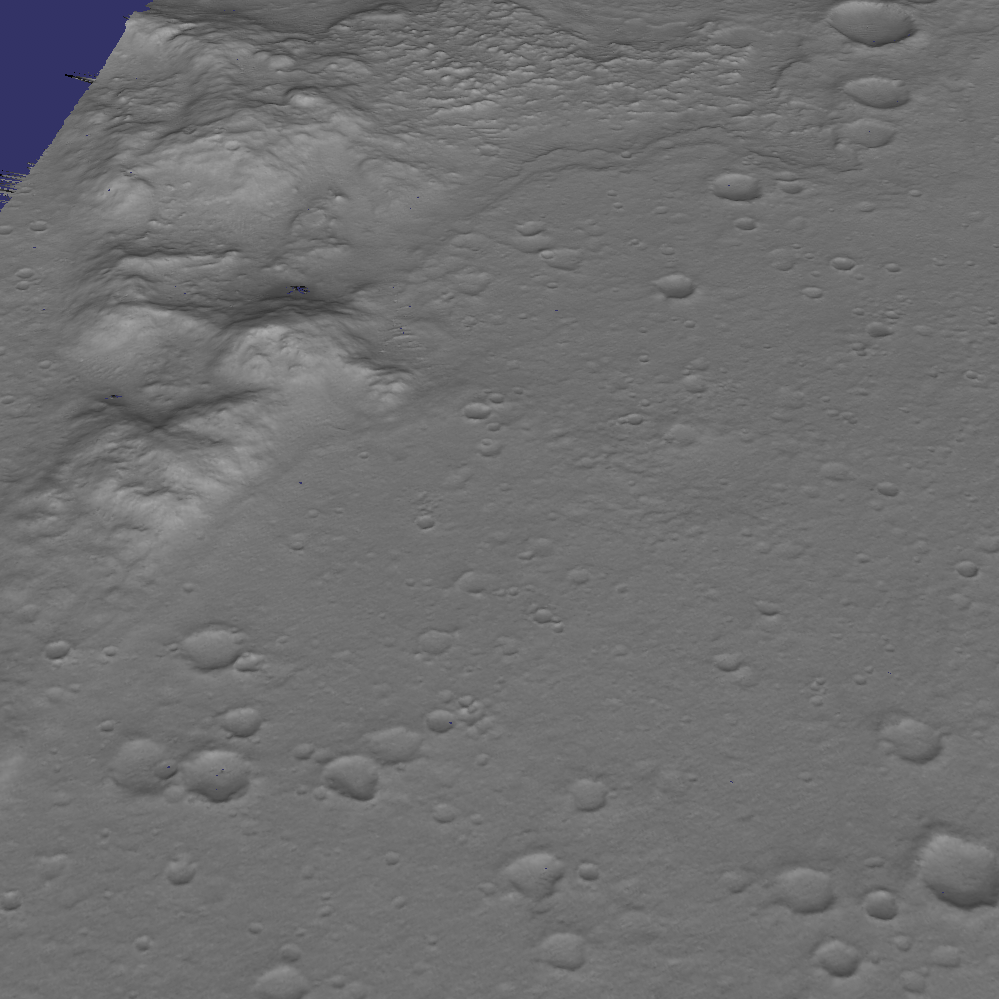
\includegraphics[width=3in]{images/examples/hirise/chills_hirise_example.png}}
  \hfil
  \subfigure[{\tt KML Screenshot}]{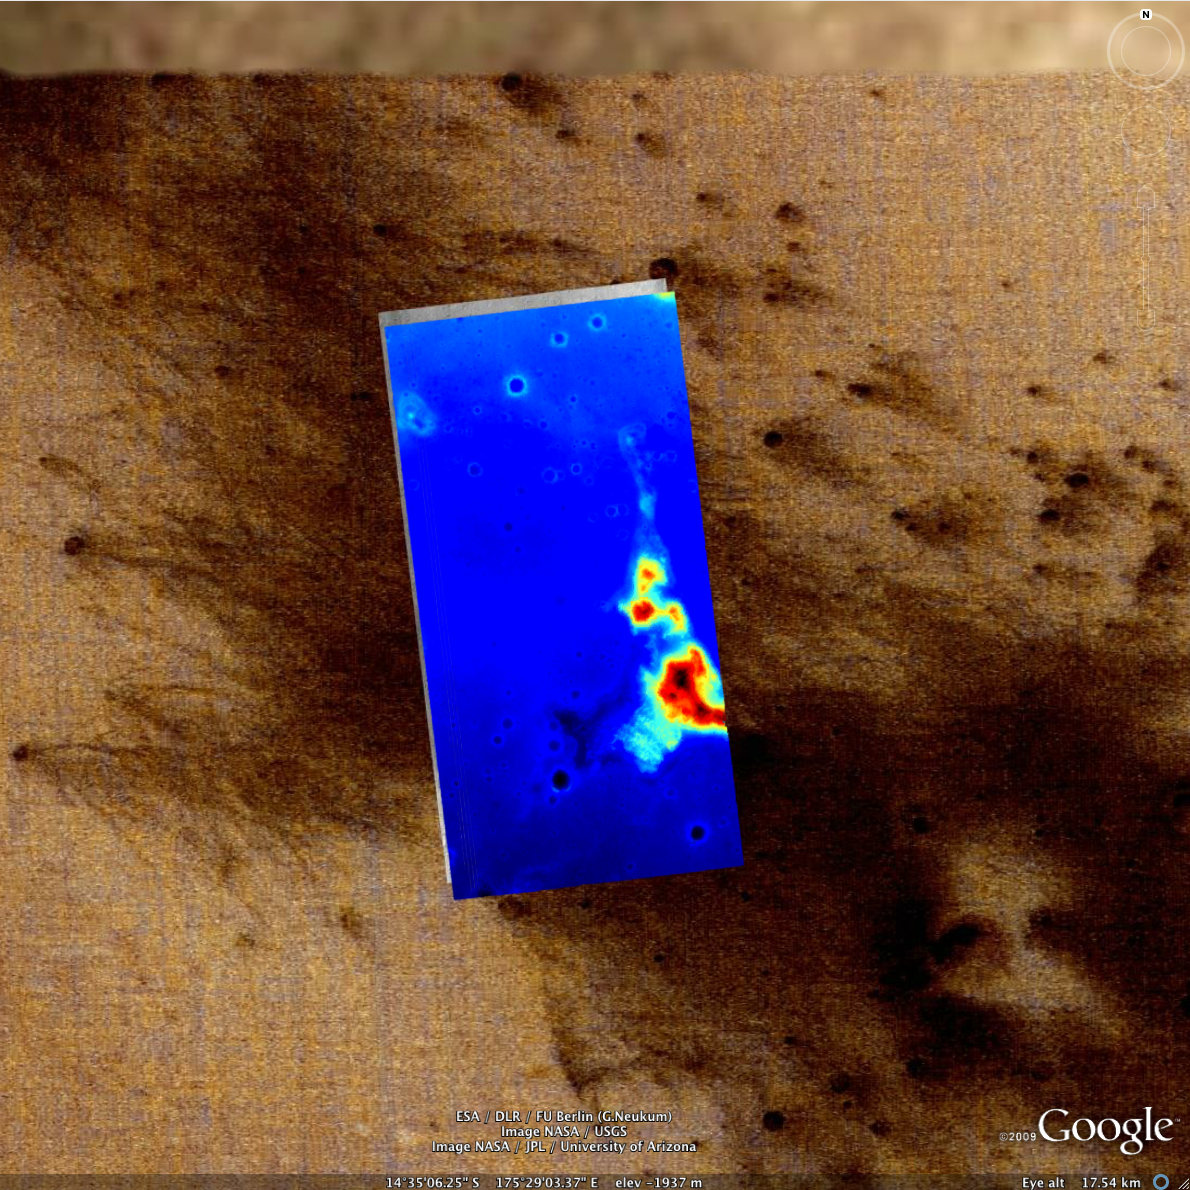
\includegraphics[width=3in]{images/examples/hirise/chills_hirise_ge_example.png}}
\caption{Example output using HiRISE images PSP\_001513\_1655 and
  PSP\_001777\_1650 of the Columbia Hills.}
\label{fig:hirise_chills_example}
\end{figure}

\subsubsection*{Commands}

Download all 20 of the RED EDR \texttt{.IMG} files for each observation.
\begin{verbatim}
  ISIS 3> hiedr2mosaic.py PSP_001513_1655_RED*.IMG
  ISIS 3> hiedr2mosaic.py PSP_001777_1650_RED*.IMG
  ISIS 3> cam2map4stereo.py PSP_001777_1650_RED.mos_hijitreged.norm.cub \
                            PSP_001513_1655_RED.mos_hijitreged.norm.cub
  ISIS 3> bandnorm from=PSP_001513_1655_RED.map.cub \
                     to=PSP_001513_1655_RED.map.norm.cub
  ISIS 3> bandnorm from=PSP_001777_1650_RED.map.cub \
                     to=PSP_001777_1650_RED.map.norm.cub
  ISIS 3> rm *RED.map.cub
  ISIS 3> mkdir result
  ISIS 3> stereo PSP_001513_1655.map.norm.cub \
                 PSP_001777_1650.map.norm.cub result/output
\end{verbatim}

\subsubsection*{stereo.default}

The stereo.default example file should apply well to HiRISE. The
\texttt{corr-kernel} value can usually be safely reduced to 21 pixels to
resolve finer detail and faster processing for images with good
contrast.

\clearpage
\subsection{East Mareotis Tholus}

%% \begin{tabular}{l r c r c}
%% \textit{Prepping Files:}       & Wall Time & \texttt{04:02:11.00} & CPU Time & \texttt{04:05:26.81} \\
%% \textit{Processing in Stereo:} & Wall Time & \texttt{59:51:01.00} & CPU Time & \texttt{164:55:02.36} \\
%% \end{tabular}

\ac{HiRISE} observations
\href{http://hirise.lpl.arizona.edu/PSP_001760_2160}{PSP\_001760\_2160} and
\href{http://hirise.lpl.arizona.edu/PSP_001364_2160}{PSP\_001364\_2160} 
cover East Mareotis Tholus, a small volcano in Tempe Terra.

\begin{figure}[h!]
\centering
  \subfigure[{\tt 3D Rendering}]{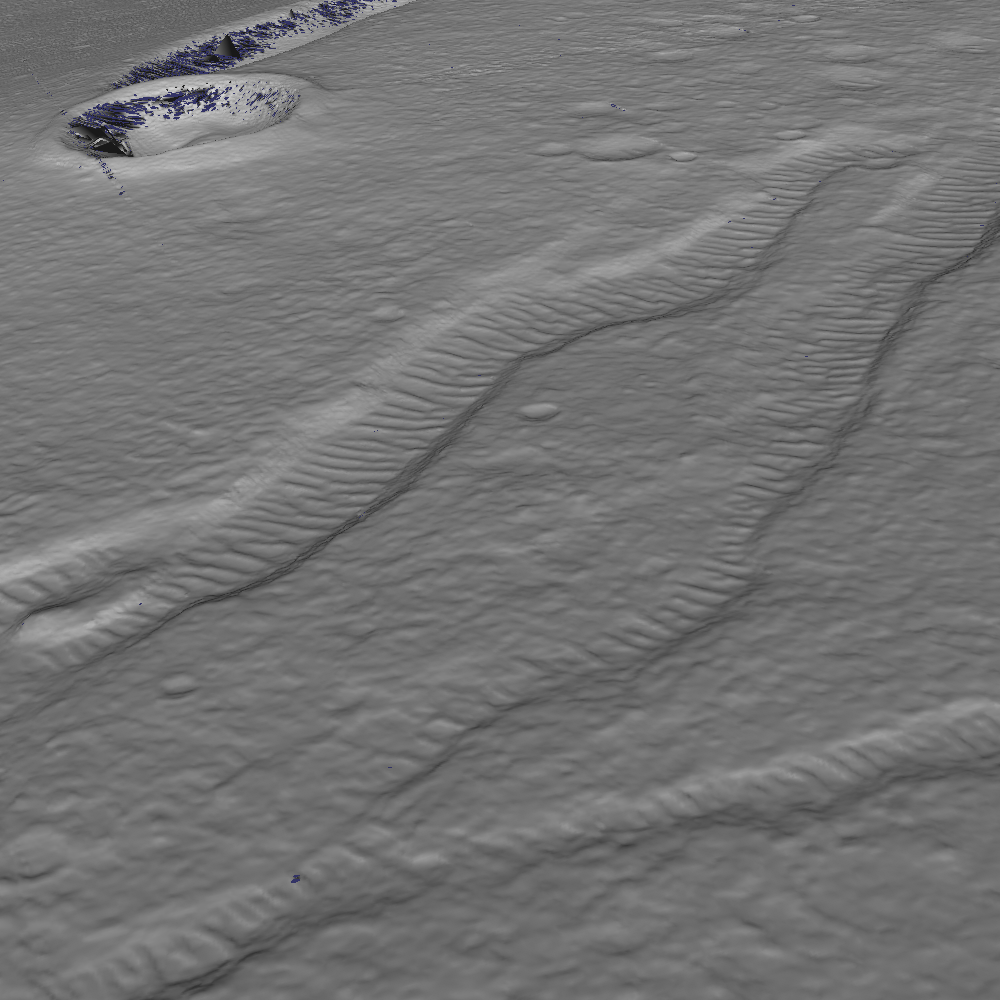
\includegraphics[width=3in]{images/examples/hirise/emare_example.png}}
  \hfil
  \subfigure[{\tt KML Screenshot}]{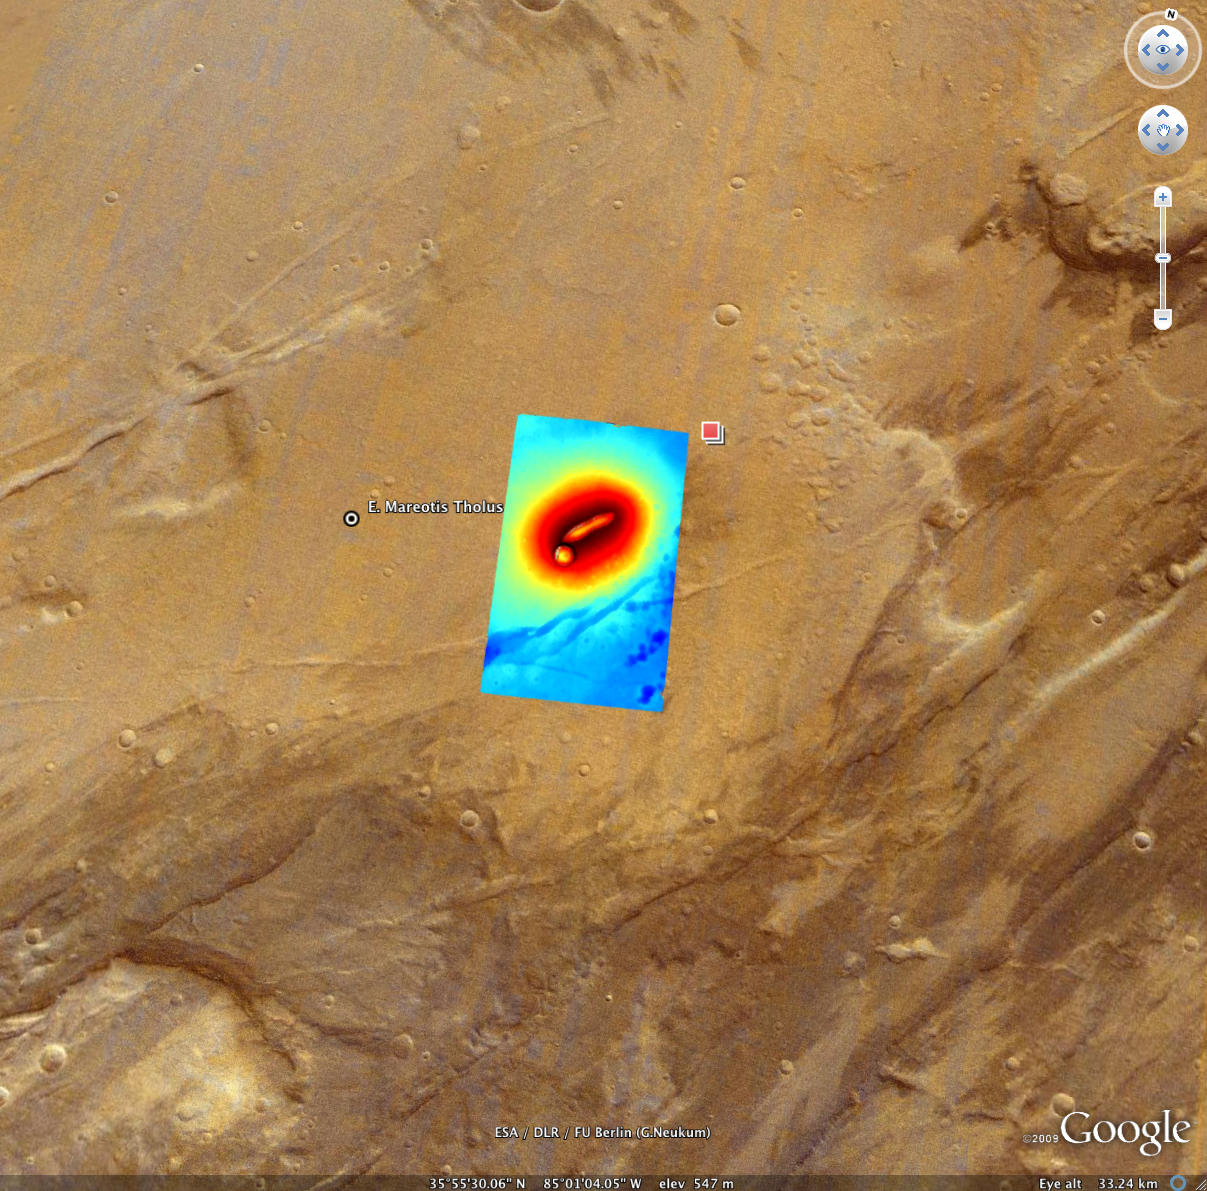
\includegraphics[width=3in]{images/examples/hirise/emare_ge_example.png}}
\caption{Example output using HiRISE images PSP\_001364\_2160 and
  PSP\_001760\_2160 of East Mareotis Tholus.}
\label{fig:hirise_emare_example}
\end{figure}

\subsubsection*{Commands}

Download all 20 of the RED EDR \texttt{.IMG} files for each observation.
\begin{verbatim}
  ISIS 3> hiedr2mosaic.py PSP_001364_2160_RED*.IMG
  ISIS 3> hiedr2mosaic.py PSP_001760_2160_RED*.IMG
  ISIS 3> cam2map4stereo.py PSP_001364_2160_RED.mos_hijitreged.norm.cub \
                            PSP_001760_2160_RED.mos_hijitreged.norm.cub
  ISIS 3> bandnorm from=PSP_001364_2160_RED.map.cub \
                     to=PSP_001364_2160_RED.map.norm.cub
  ISIS 3> bandnorm from=PSP_001760_2160_RED.map.cub \
                     to=PSP_001760_2160_RED.map.norm.cub
  ISIS 3> ls *.map.norm.cub > fromlist
  ISIS 3> ls *1760*.map.norm.cub > holdlist
  ISIS 3> equalizer fromlist=fromlist holdlist=holdlist
  ISIS 3> rm *RED.map.norm.cub *RED.map.cub
  ISIS 3> mkdir result
  ISIS 3> stereo PSP_001364_2160.map.norm.equ.cub \
                 PSP_001760_2160.map.norm.equ.cub result/output
\end{verbatim}

\subsubsection*{stereo.default}

The stereo.default example file should apply well to HiRISE. The
\texttt{corr-kernel} parameter can usually be safely reduced to 21
pixels to resolve finer detail and faster processing for images
with good contrast.

\clearpage
\subsection{North Terra Meridiani Crop}

\ac{HiRISE} observations
\href{http://hirise.lpl.arizona.edu/PSP_001981_1825}{PSP\_001981\_1825} and
\href{http://hirise.lpl.arizona.edu/PSP_002258_1825}{PSP\_002258\_1825}
show a small crater filled by layered material.

\begin{figure}[h!]
\centering
  \subfigure[{\tt 3D Rendering}]{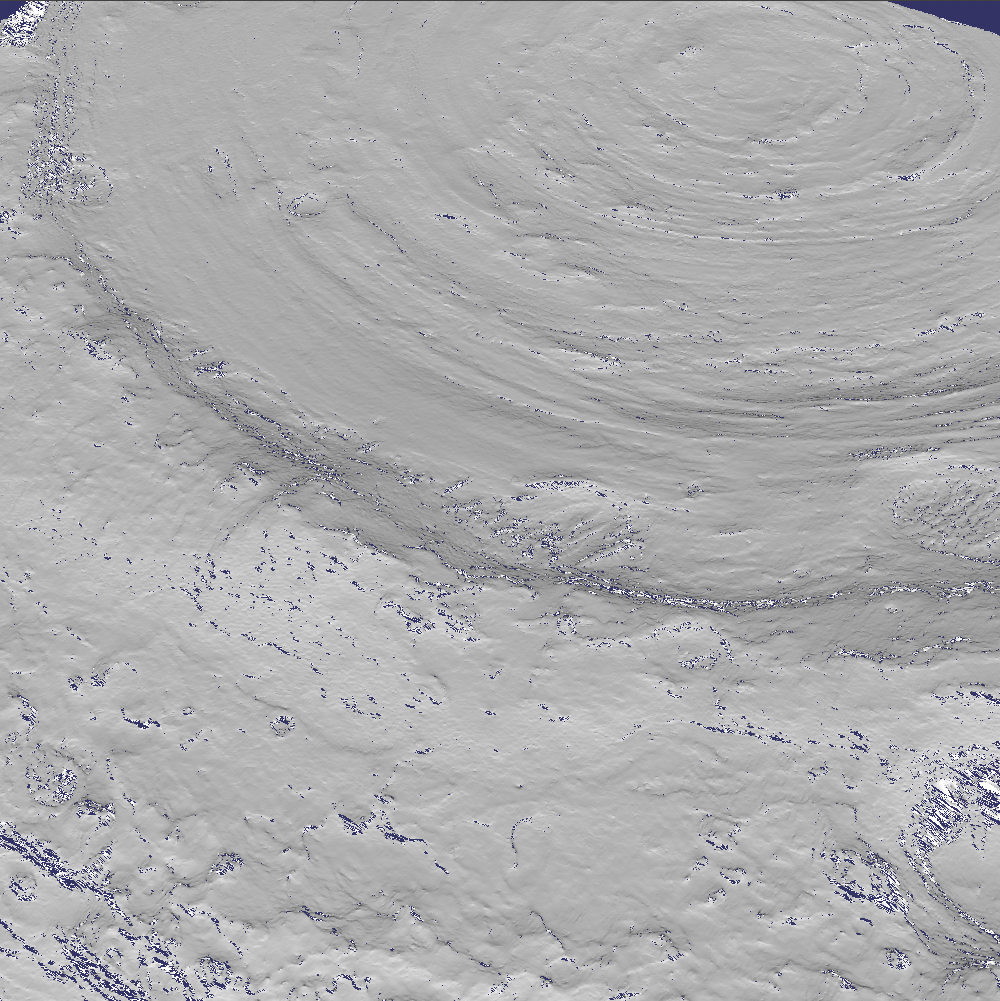
\includegraphics[height=2.5in]{images/examples/hirise/nterra_example.png}}
  \hfil
  \subfigure[{\tt KML Screenshot}]{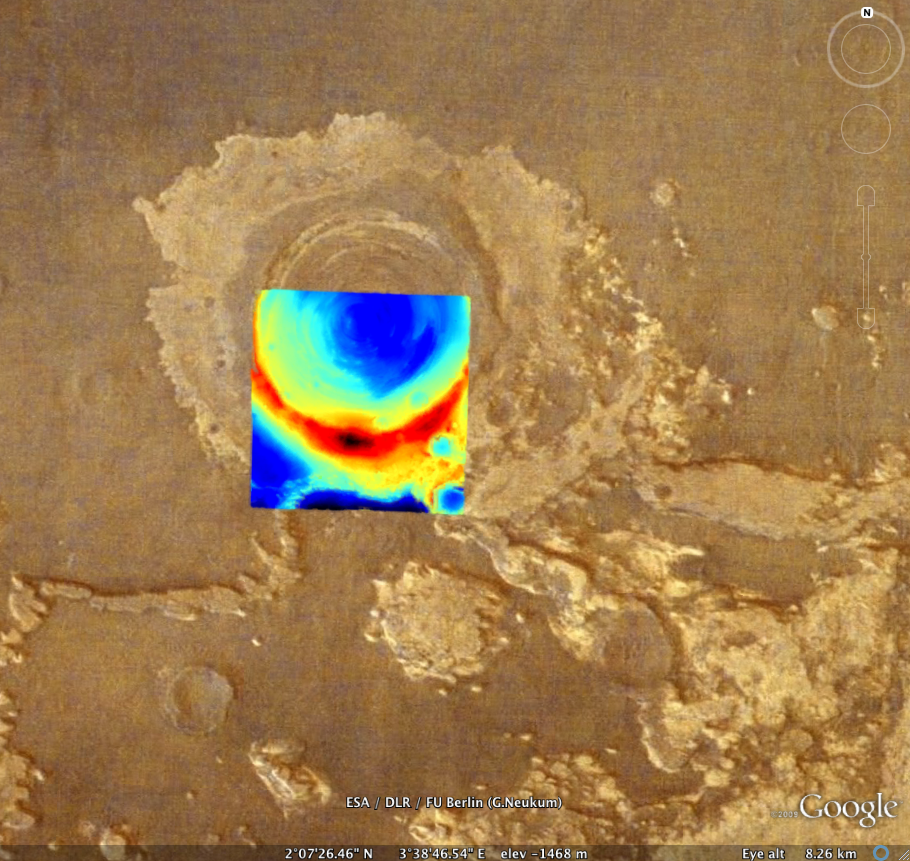
\includegraphics[height=2.5in]{images/examples/hirise/nterra_ge_example.png}}
\caption{Example output using cropped HiRISE data of North Terra Meridiani.}
\label{fig:hirise_nterra_example}
\end{figure}

\subsubsection*{Commands}

Notice here that we have applied a crop to select a subset of these
HiRISE images that we are interested in.  Cropping is often an
efficient way to go because it greatly reduces the amount of
computation necessary to get results in a limited area.  As always,
Download all 20 of the RED EDR \texttt{.IMG} files for each observation.
\begin{verbatim}
  ISIS 3> hiedr2mosaic.py PSP_001981_1825_RED*.IMG
  ISIS 3> hiedr2mosaic.py PSP_002258_1825_RED*.IMG
  ISIS 3> cam2map from=PSP_001981_1825_RED.mos_hijitreged.norm.cub \
                    to=PSP_001981_1825_REDmosaic.map.cub
  ISIS 3> cam2map from=PSP_002258_1825_RED.mos_hijitreged.norm.cub \
                   map=PSP_001981_1825_REDmosaic.map.cub \
                    to=PSP_002258_1825_REDmosaic.map.cub matchmap=true
  ISIS 3> bandnorm from=PSP_001981_1825_REDmosaic.map.cub \
                     to=PSP_001981_1825_REDmosaic.map.norm.cub
  ISIS 3> bandnorm from=PSP_002258_1825_REDmosaic.map.cub \
                     to=PSP_002258_1825_REDmosaic.map.norm.cub
  ISIS 3> ls *.map.norm.cub > fromlist
  ISIS 3> ls *1981*.map.norm.cub > holdlist
  ISIS 3> equalizer fromlist=fromlist holdlist=holdlist
  ISIS 3> crop from=PSP_001981_1825_REDmosaic.map.norm.equ.cub \
                 to=PSP_001981_1825.crop.cub sample=7497 line=41318 nsamp=10000 nline=10000
  ISIS 3> crop from=PSP_002258_1825_REDmosaic.map.norm.equ.cub \
                 to=PSP_002258_1825.crop.cub sample=7982 line=41310 nsamp=10000 nline=10000
  ISIS 3> rm *REDmosaic*.cub
  ISIS 3> mkdir result
  ISIS 3> stereo PSP_001981_1825.crop.cub PSP_002258_1825.crop.cub result/output
\end{verbatim}

\subsubsection*{stereo.default}

The stereo.default example file should apply well to HiRISE. The
\texttt{corr-kernel} value can usually be safely reduced to 21 pixels to
resolve finer detail and faster processing for images with good
contrast.

\vfill

\section{Mars Reconnaissance Orbiter CTX}

\ac{CTX} is a moderate camera to work with. Processing times for
\ac{CTX} can be pretty long when using Bayes EM subpixel
refinement. Otherwise the disparity between images is relatively
small, allowing efficient computation and a reasonable processing time.

\subsection{North Terra Meridiani}

%% \begin{tabular}{l r c r c}
%% \textit{Processing in Stereo:} & Wall Time & \texttt{13:28:04.00} & CPU Time & \texttt{45:54:50.10} \\
%% \end{tabular}

In this example, we use map projected images. Map projecting the
images is the most reliable way to align the images for
correlation. However when possible, use non-map-projected images with
the \texttt{alignment-method homography} option. This greatly reduces
the time spent in triangulation. For all cases using linescan cameras,
triangulation of map-projected images is 10x slower than
non-map-projected images.

This example is distributed in the \texttt{examples/CTX} directory.

\begin{figure}[b!]
\centering
  \subfigure[{\tt 3D Rendering}]{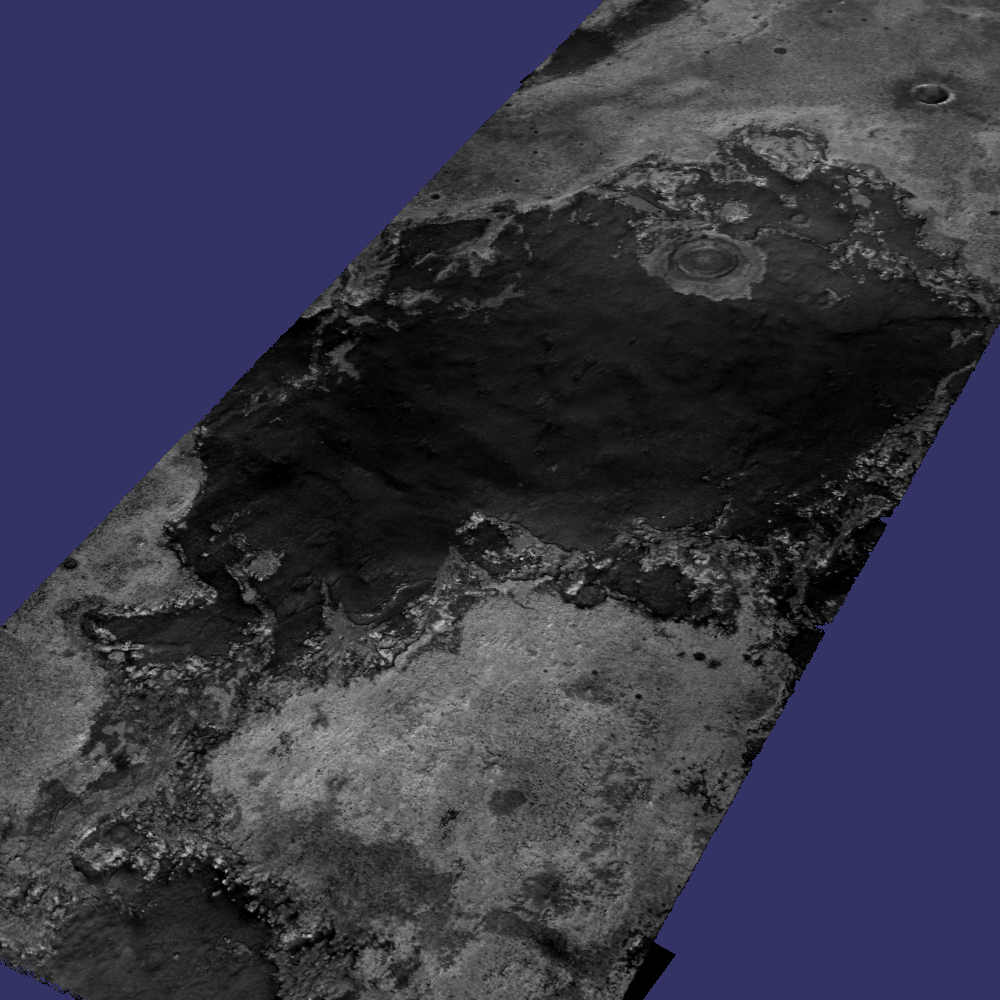
\includegraphics[width=3in]{images/examples/ctx/n_terra_meridiani_ctx.png}}
  \hfil
  \subfigure[{\tt KML Screenshot}]{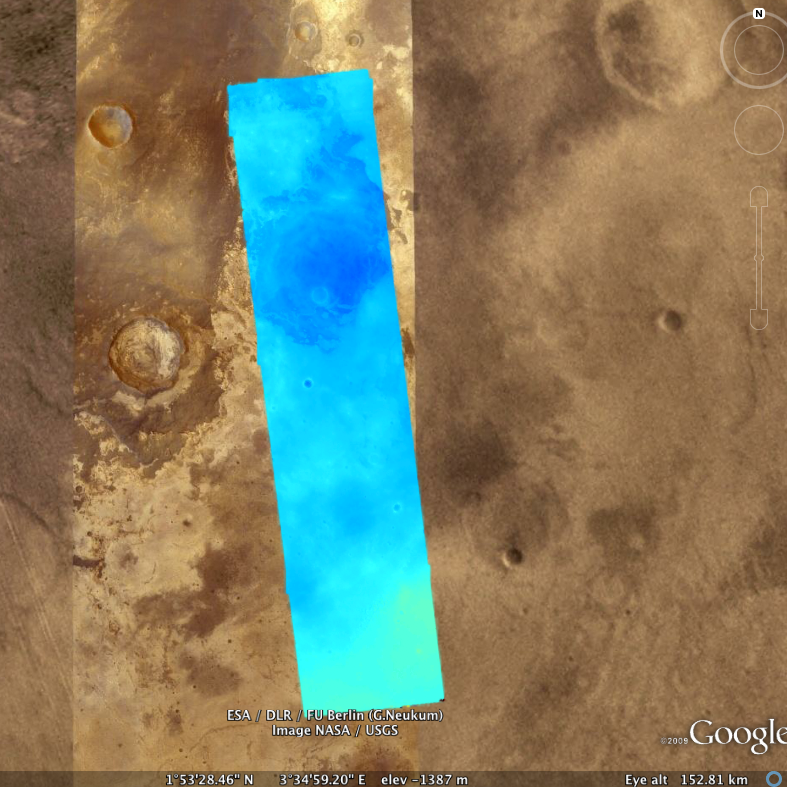
\includegraphics[width=3in]{images/examples/ctx/n_terra_meridiani_ctx_ge.png}}
\caption{Example output possible with the CTX imager aboard MRO.}
\label{fig:ctx_example}
\end{figure}

\subsubsection*{Commands}

Download the \ac{CTX} images P02\_001981\_1823\_XI\_02N356W.IMG and
P03\_002258\_1817\_XI\_01N356W.IMG from the \ac{PDS}.
\begin{Verbatim}[commandchars=\\\{\}]
  ISIS 3> mroctx2isis from=P02_001981_1823_XI_02N356W.IMG to=P02_001981_1823.cub
  ISIS 3> mroctx2isis from=P03_002258_1817_XI_01N356W.IMG to=P03_002258_1817.cub
  ISIS 3> spiceinit from=P02_001981_1823.cub
  ISIS 3> spiceinit from=P03_002258_1817.cub
  ISIS 3> ctxcal from=P02_001981_1823.cub to=P02_001981_1823.cal.cub
  ISIS 3> ctxcal from=P03_002258_1817.cub to=P03_002258_1817.cal.cub
    \textnormal{you can also optionally run} ctxevenodd \textnormal{on the} cal.cub \textnormal{files, if needed}
  ISIS 3> cam2map4stereo.py P02_001981_1823.cal.cub P03_002258_1817.cal.cub
  ISIS 3> mkdir result
  ISIS 3> stereo P02_001981_1823.map.cub P03_002258_1817.map.cub results/out
\end{Verbatim}

\subsubsection*{stereo.default}

The stereo.default example file works generally well with all CTX pairs.

\clearpage
\section{Mars Global Surveyor MOC-NA}

In the Stereo Pipeline Tutorial in Chapter~\ref{ch:tutorial}, we
showed you how to process a narrow angle \ac{MOC} stereo pair that
covered a portion of Hrad Vallis. In this section we will show you
more examples, some of which exhibit a problem common to stereo
pairs from linescan imagers: ``spacecraft jitter'' is caused by
oscillations of the spacecraft due to the movement of other spacecraft
hardware.  All spacecraft wobble around to some degree but some are 
particularly susceptible.

Jitter causes wave-like distortions along the track of the satellite
orbit in \acp{DEM} produced from linescan camera images.  This effect can
be very subtle or quite pronounced, so it is important to check your
data products carefully for any sign of this type of artifact. The
following examples will show the typical distortions created by this
problem.

Note that the science teams of \ac{HiRISE} and \ac{LROC} are actively
working on detecting and correctly modeling jitter in their respective
SPICE data. If they succeed in this, the distortions will still
be present in the raw imagery, but the jitter will no longer produce
ripple artifacts in the DEMs produced using ours or other stereo
reconstruction software.

\subsection{Ceraunius Tholus}

%% \begin{tabular}{l r c r c}
%% \textit{Prepping Files:}       & Wall Time & \texttt{00:02:42.30} & CPU Time & \texttt{00:02:42.06} \\
%% \textit{Processing in Stereo:} & Wall Time & \texttt{00:23:00.30} & CPU Time & \texttt{00:34:11.00} \\
%% \end{tabular}

Ceraunius Tholus is a volcano in northern Tharsis on Mars. It can
be found at 23.96 N and 262.60 E. This \ac{DEM} crosses the volcano's
caldera.

\begin{figure}[h]
\centering
  \subfigure[{\tt 3D Rendering}]{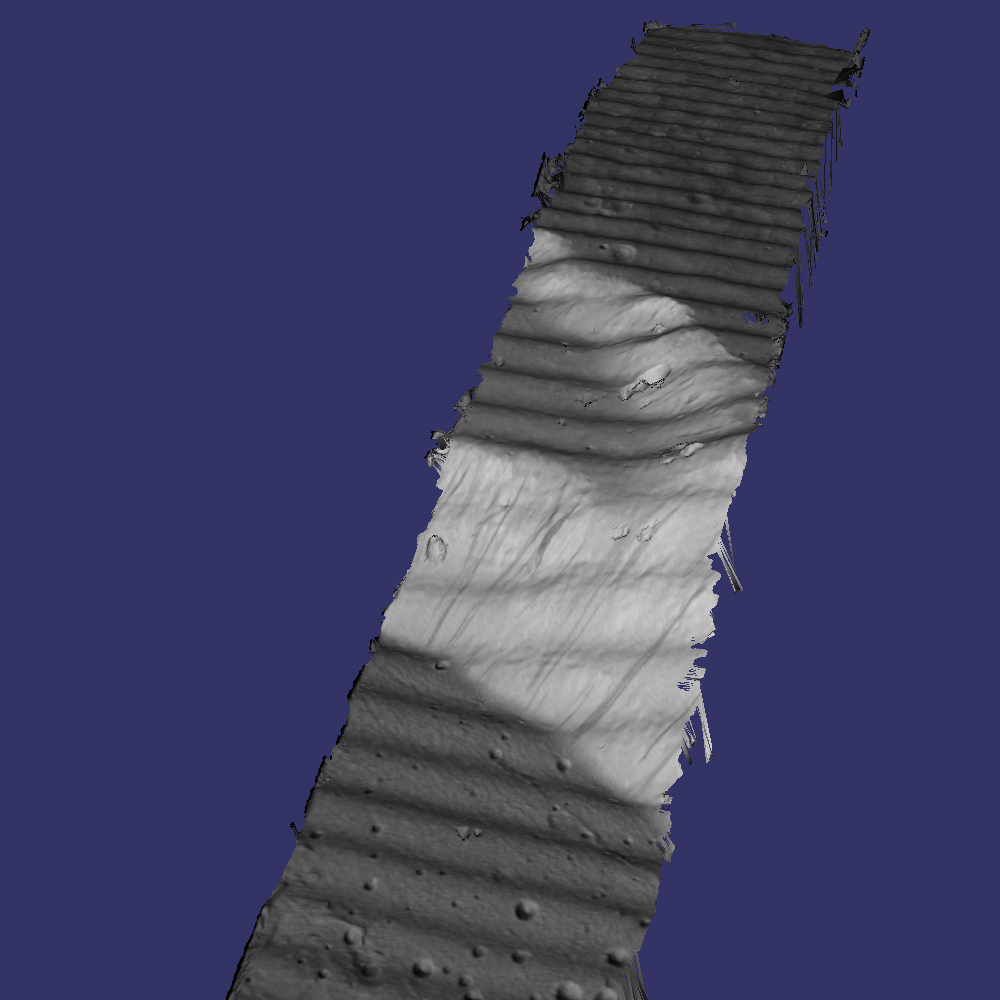
\includegraphics[width=3in]{images/examples/mocna/ceraunius_tholus_mocna.png}}
  \hfil
  \subfigure[{\tt KML Screenshot}]{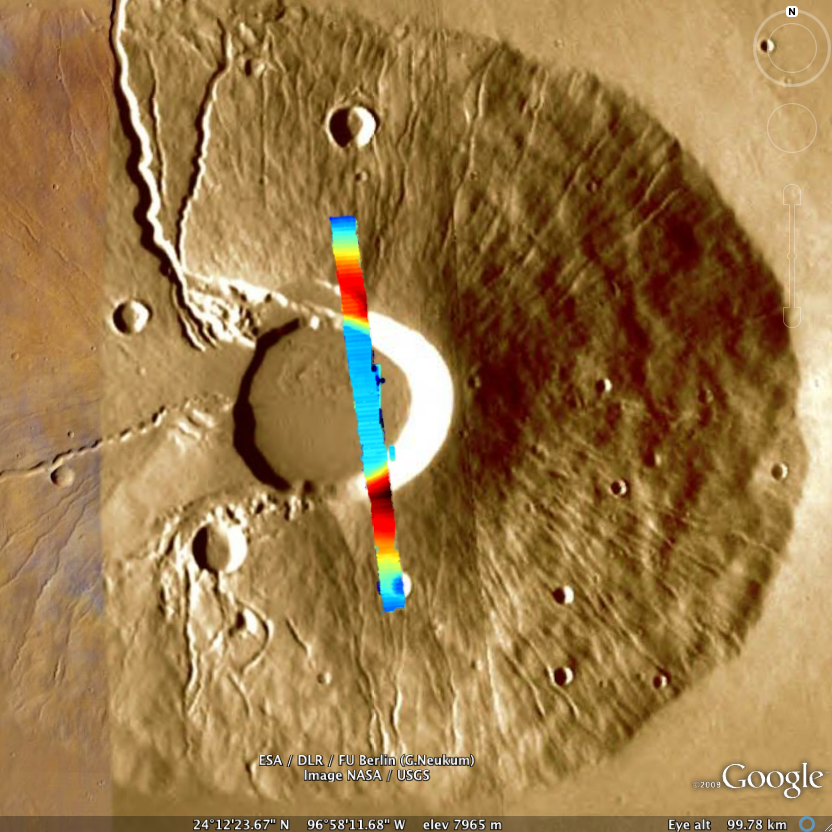
\includegraphics[width=3in]{images/examples/mocna/ceraunius_tholus_mocna_ge.png}}
\caption{Example output for MOC-NA of Ceraunius Tholus. Notice the presence of severe washboarding artifacts due to spacecraft ``jitter.''}
\label{fig:mocna_ceraunius_example}
\end{figure}

\subsubsection*{Commands}

Download the M08/06047 and R07/01361 images from the \ac{PDS}.

\begin{verbatim}
  ISIS 3> moc2isis f=M0806047.img t=M0806047.cub
  ISIS 3> moc2isis f=R0701361.img t=R0701361.cub
  ISIS 3> spiceinit from=M0806047.cub
  ISIS 3> spiceinit from=R0701361.cub
  ISIS 3> cam2map4stereo.py M0806047.cub R0701361.cub
  ISIS 3> mkdir result
  ISIS 3> stereo M0806047.map.cub R0701361.map.cub result/output
\end{verbatim}

\subsubsection*{stereo.default}

The stereo.default example file works generally well with all MOC-NA pairs.

\newpage
\subsection{North Tharsis}

%% \begin{tabular}{l r c r c}
%% \textit{Prepping Files:}       & Wall Time & \texttt{00:01:57.52} & CPU Time & \texttt{00:01:56.79} \\
%% \textit{Processing in Stereo:} & Wall Time & \texttt{00:24:50.70} & CPU Time & \texttt{01:34:37.40} \\
%% \end{tabular}

These images cover troughs and terraces in northern Tharsis.
This \ac{DEM} is located at 20.20 N and 118.18 W on Mars.

\begin{figure}[h!]
\centering
  \subfigure[{\tt 3D Rendering}]{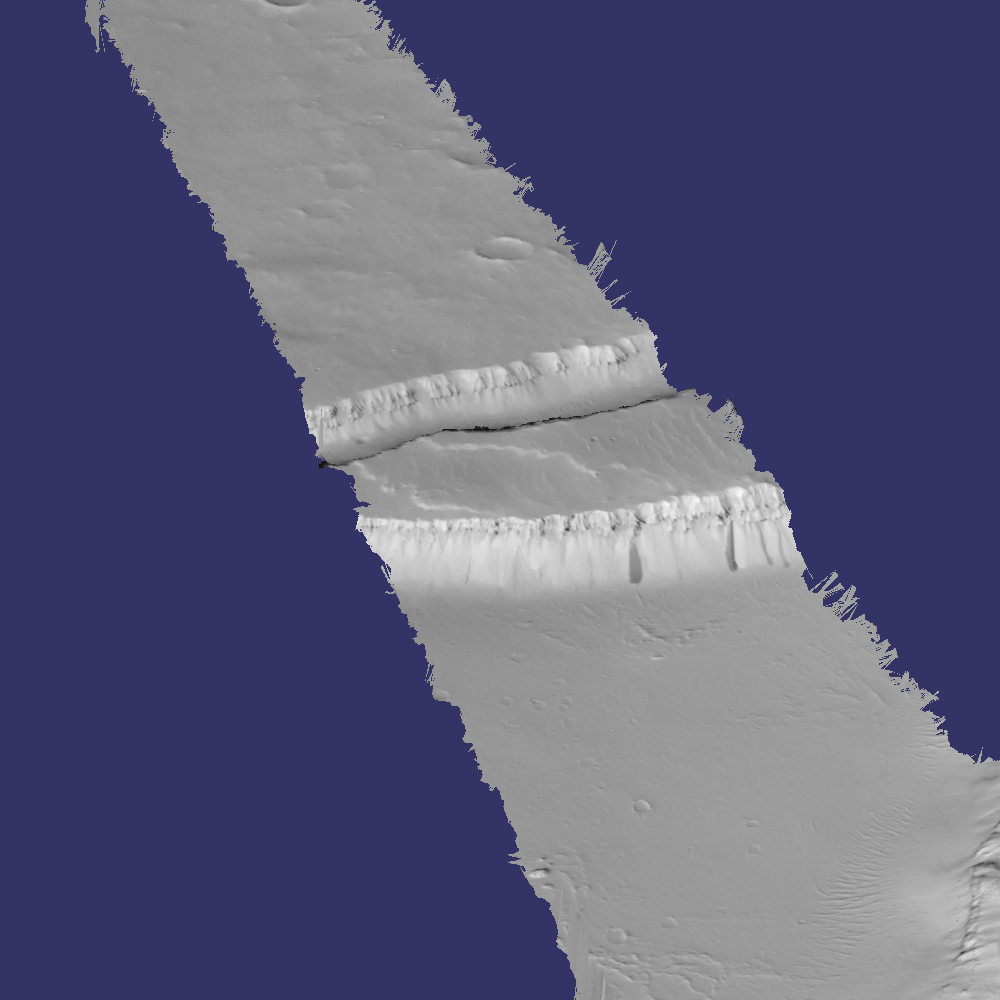
\includegraphics[width=3in]{images/examples/mocna/n_tharsis_mocna.png}}
  \hfil
  \subfigure[{\tt KML Screenshot}]{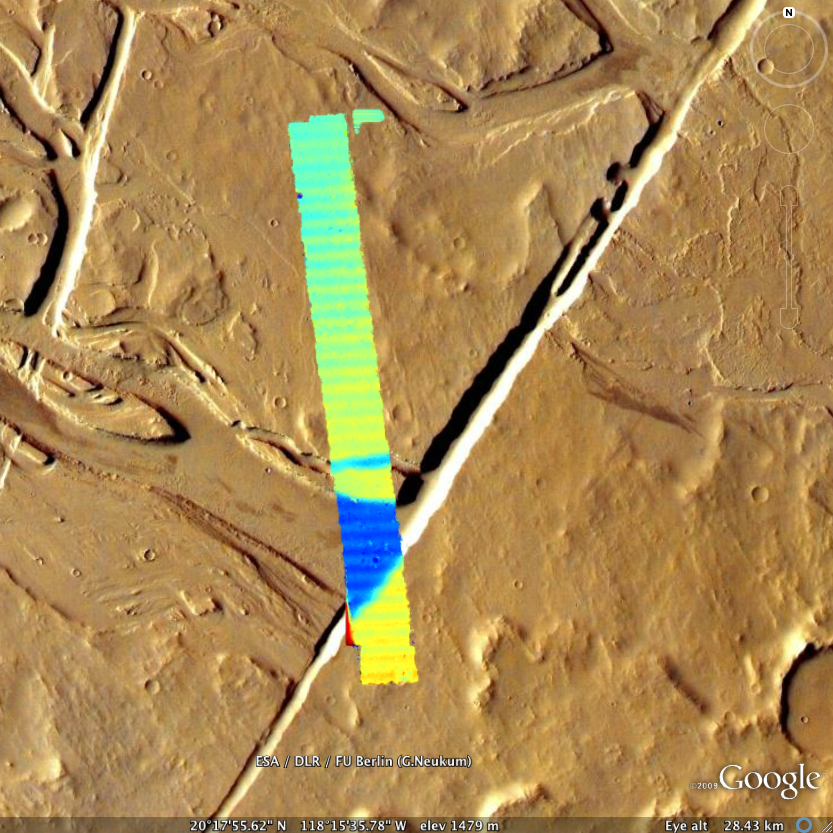
\includegraphics[width=3in]{images/examples/mocna/n_tharsis_mocna_ge.png}}
\caption{Example output for MOC-NA of North Tharsis.}
\label{fig:mocna_n_tharsis_example}
\end{figure}

\subsubsection*{Commands}

Download the M08/03097.img and S07/01420 images from the \ac{PDS}.
\begin{verbatim}
  ISIS 3> moc2isis f=M0803097.img t=M0803097.cub
  ISIS 3> moc2isis f=S0701420.img t=S0701420.cub
  ISIS 3> cam2map4stereo.py M0803097.cub S0701420.cub
  ISIS 3> mkdir result
  ISIS 3> stereo M0803097.map.cub S0701420.map.cub result/output
\end{verbatim}

\subsubsection*{stereo.default}

The stereo.default example file works generally well with all MOC-NA pairs.

\newpage
\section{Mars Exploration Rovers MER}

The MER rovers have several cameras on board and they all seem to have
a stereo pair. With ASP you are able to process the PANCAM, NAVCAM,
and HAZCAM camera imagery. ISIS has no telemetry or camera instrinsic
supports for these images. That however is not a problem as their raw
imagery contains the cameras' information in JPL's CAHV, CAHVOR, and
CHAVORE formats.

These cameras are all variations of a simple pinhole camera model so
they are processed with ASP in the \texttt{PINHOLE} session instead of
the usual \texttt{ISIS}. ASP only supports creating of point
clouds. \emph{The *-PC.tif is a raw point cloud with the first 3
  channels being XYZ in the rover site's coordinate frame}. We don't
support the creation of DEMs from these images and that is left as an
excercise for the user.

\subsection{PANCAM, NAVCAM, HAZCAM}

All of these cameras are processed the same way. I'll be showing 3D
processing of the front hazard cams. The only new things in the
pipeline is the new executable \texttt{mer2camera} along with the use
of \texttt{alignment-method epipolar}. This example is also provided
in the MER data example directory.

\begin{figure}[h!]
\centering
  \subfigure[{\tt Rectified Input}]{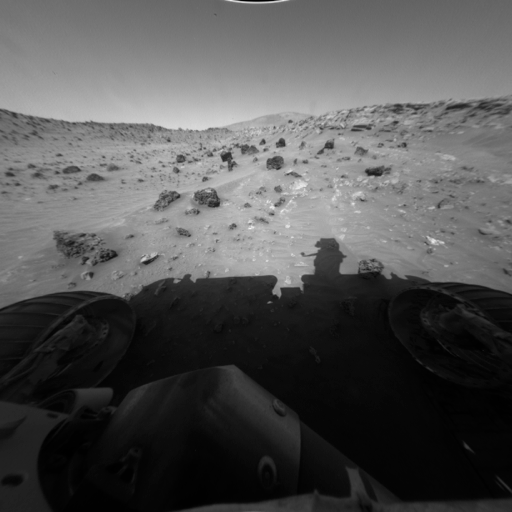
\includegraphics[width=3in]{images/examples/mer/fh01-L_sub.png}}
  \hfil
  \subfigure[{\tt Output Point Cloud}]{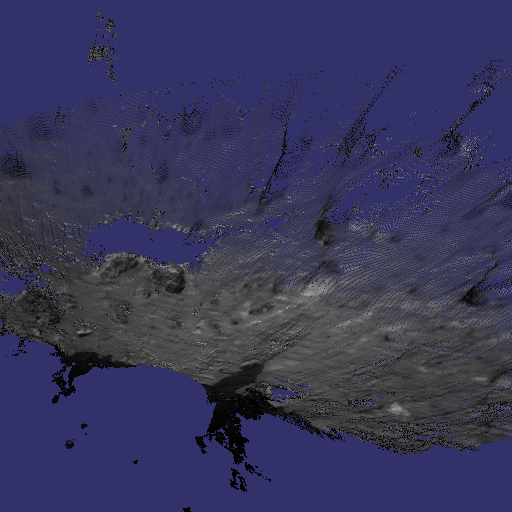
\includegraphics[width=3in]{images/examples/mer/fh01_pointcloud.png}}
\caption{Example output possible with the front hazard cameras.}
\label{fig:metric_example}
\end{figure}

\pagebreak

\subsubsection*{Commands}

Download 2f194370083effap00p1214l0m1.img and
2f194370083effap00p1214r0m1.img from the \ac{PDS}.

\begin{verbatim}
  ISIS 3> gdal_translate -scale -ot byte 2f194370083effap00p1214l0m1.img \
                                         2f194370083effap00p1214l0m1.tif
  ISIS 3> gdal_translate -scale -ot byte 2f194370083effap00p1214r0m1.img \
                                         2f194370083effap00p1214r0m1.tif
  ISIS 3> mer2camera 2f194370083effap00p1214l0m1.img
  ISIS 3> mer2camera 2f194370083effap00p1214r0m1.img
  ISIS 3> stereo 2f194370083effap00p1214l0m1.tif 2f194370083effap00p1214r0m1.tif \
                 2f194370083effap00p1214l0m1.cahvore 2f194370083effap00p1214r0m1.cahvore \
                 fh01/fh01
\end{verbatim}

\subsection*{stereo.default}

The default stereo settings will work but change the following options:

\begin{center}\begin{minipage}{5.5in}
\begin{Verbatim}[frame=single,fontsize=\small,label=additional settings for MER]
    alignment-method EPIPOLAR
    force-use-entire-range

    # This deletes points that are too far away
    # from the camera to truly triangulate.
    universe-center Camera
    near-universe-radius 0.7
    far-universe-radius 80.0
\end{Verbatim}
\end{minipage}\end{center}

\clearpage
\section{Lunar Reconaissance Orbiter LROC NAC}

\subsection{Lee-Lincoln Scarp}

This stereo pair covers the Taurus-Littrow valley on the Moon where,
on December 11, 1972, the astronauts of Apollo 17 landed. However,
this stereo pair does not contain the landing site.  It is slightly
west; focusing on the Lee-Lincoln scarp that is on North Massif. The
scarp is an 80~m high feature that is the only visible sign of a deep
fault.

\begin{figure}[h!]
\centering
  \subfigure[{\tt 3D Rendering}]{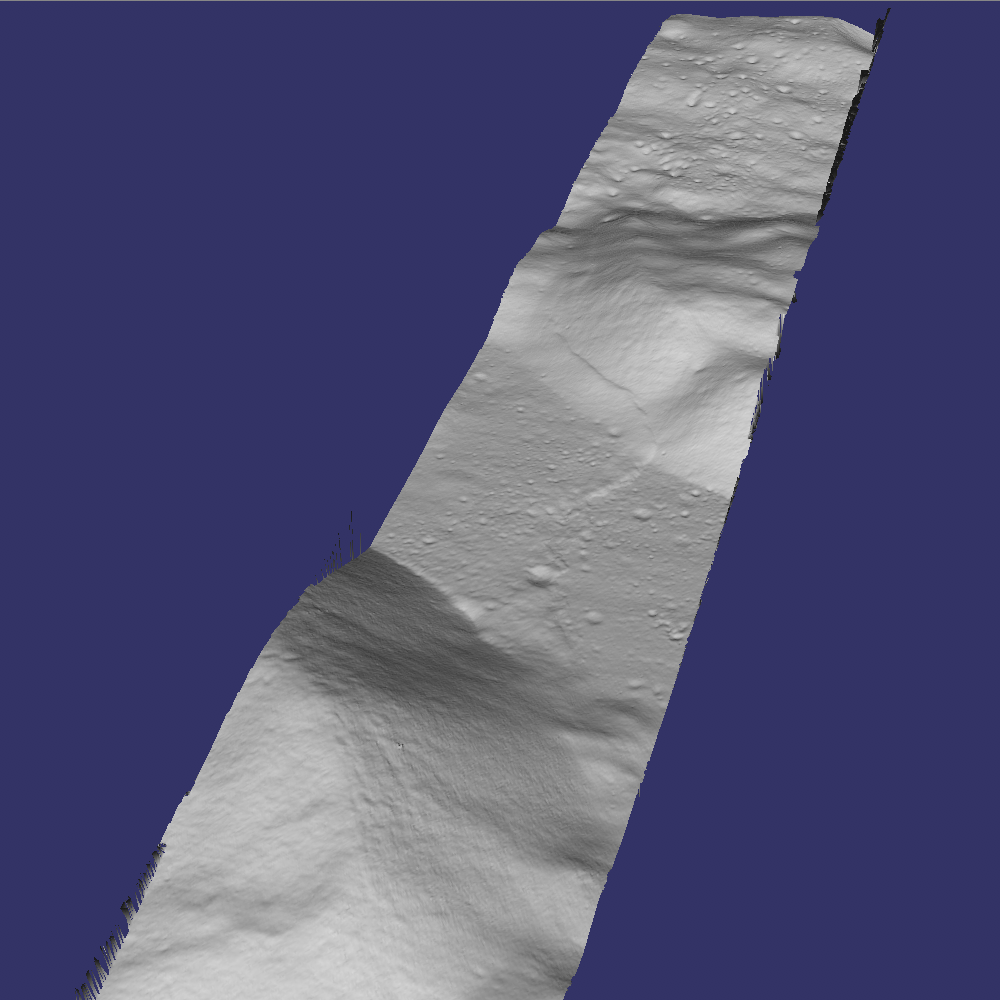
\includegraphics[width=3in]{images/examples/lrocna/lroc-na-example.png}}
  \hfil
  \subfigure[{\tt KML Screenshot}]{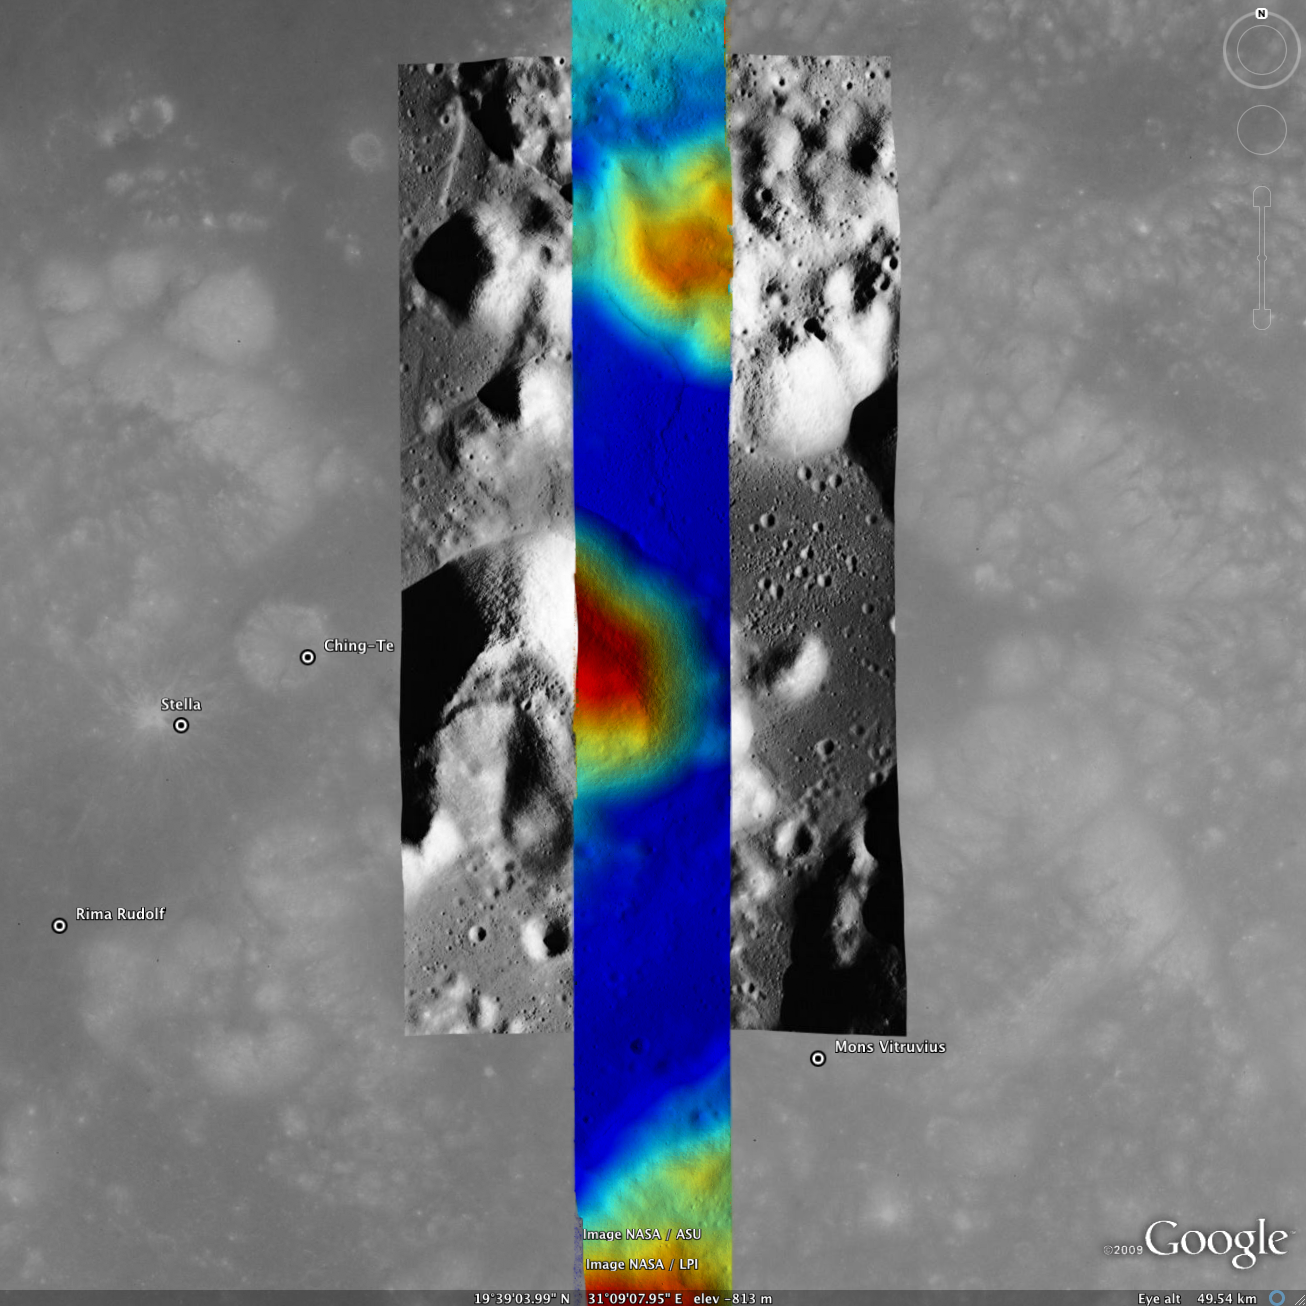
\includegraphics[width=3in]{images/examples/lrocna/lroc-na-ge_example.png}}
\caption{Example output possible with a LROC NA stereo pair, using only a single CCD from each observation.}
\label{fig:lroc-na-example}
\end{figure}

\subsubsection*{Commands}

Download the EDRs for the left CCDs for observations M104318871 and
M104318871. Alternatively you can search by original IDs of 2DB8 and
4C86 in the PDS.

\begin{verbatim}
    ISIS 3> lronac2isis from=M104318871LE.img to=M104318871LE.cub
    ISIS 3> lronac2isis from=M104311715LE.img to=M104311715LE.cub
    ISIS 3> spiceinit M104318871LE.cub
    ISIS 3> spiceinit M104311715LE.cub
    ISIS 3> lronaccal from=M104318871LE.cub to=M104318871LE.cal.cub
    ISIS 3> lronaccal from=M104311715LE.cub to=M104311715LE.cal.cub
    ISIS 3> cam2map4stereo.py M104318871LE.cal.cub M104311715LE.cal.cub
    ISIS 3> stereo M104318871LE.map.cub M104311715LE.map.cub result/output
\end{verbatim}

\subsubsection*{stereo.default}

The stereo.default example file works generally well with LRO-NAC
pairs. The recommended route for processing LRO-NAC imagery is by map
projecting them. Map-projecting with higher resolution data such as
LRO-WAC Global DTM also helps processing greatly. When map projecting,
be sure to remember to set \texttt{alignment-method NONE}.

\section{Apollo 15 Metric Camera Images}

\begin{tabular}{ r c r c}

\end{tabular}

Apollo Metric images were all taken at regular intervals, which means
that the same \texttt{stereo.default} can be used for all sequential pairs of
images. Apollo Metric images are ideal for stereo processing.  They
produce consistent, excellent results.

The scans performed by ASU are sufficiently detailed to exhibit film
grain at the highest resolution.  The amount of noise at the full
resolution is not helpful for the correlator, so we recommend
subsampling the images by a factor of 4.

Currently the tools to ingest Apollo TIFFs into ISIS are not
available, but these images should soon be released into the PDS for
general public usage.

\subsection{Ansgarius C}

%% \begin{tabular}{ r c r c}
%% \multicolumn{3}{l}{ \emph{Prepping Files} } \\
%% Wall Time & \texttt{00:00:02.11} & CPU Time & \texttt{00:00:01.29} \\
%% \multicolumn{3}{l}{ \emph{Processing in Stereo} } \\
%% Wall Time & \texttt{01:52:23.00} & CPU Time & \texttt{21:36:07.61} \\
%% \end{tabular}

Ansgarius C is a small crater on the west edge of the farside of the
Moon near the equator. It is east of Kapteyn A and B.

\begin{figure}[h!]
\centering
  \subfigure[{\tt 3D Rendering}]{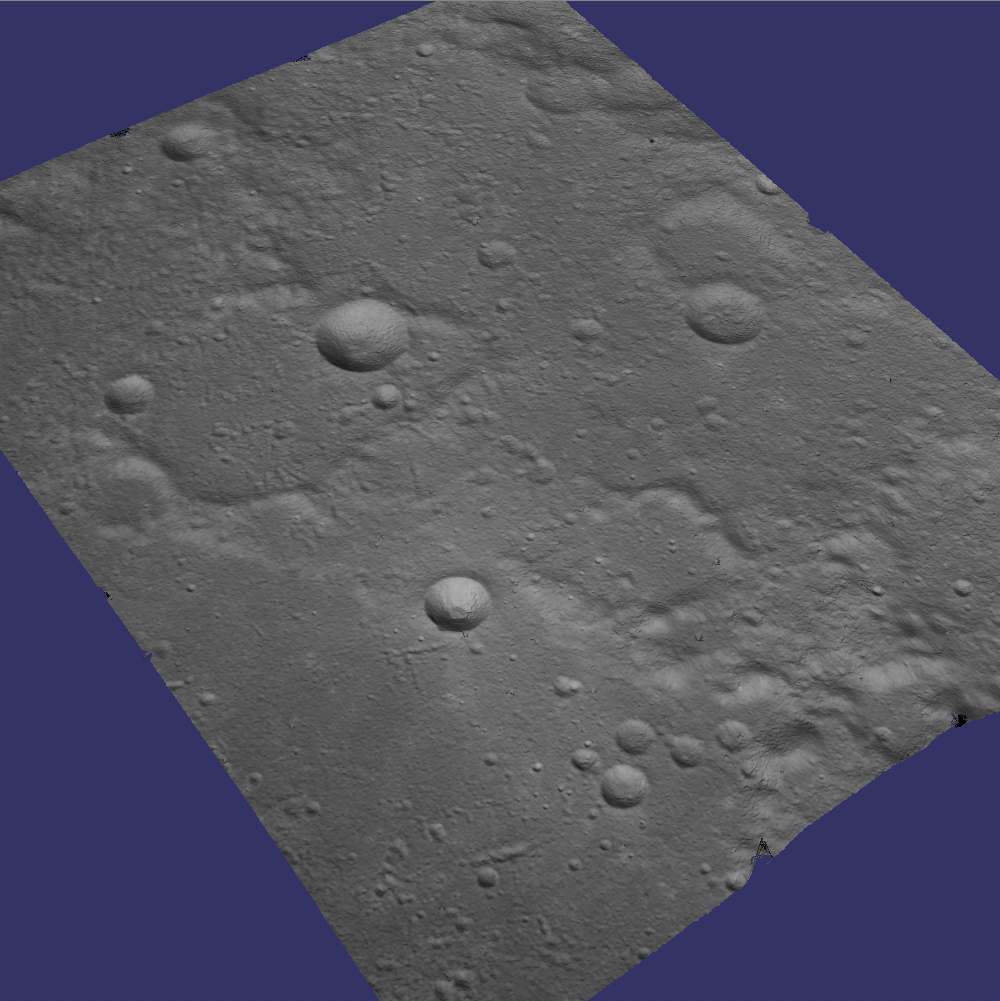
\includegraphics[width=3in]{images/examples/metric/metric_example.png}}
  \hfil
  \subfigure[{\tt KML Screenshot}]{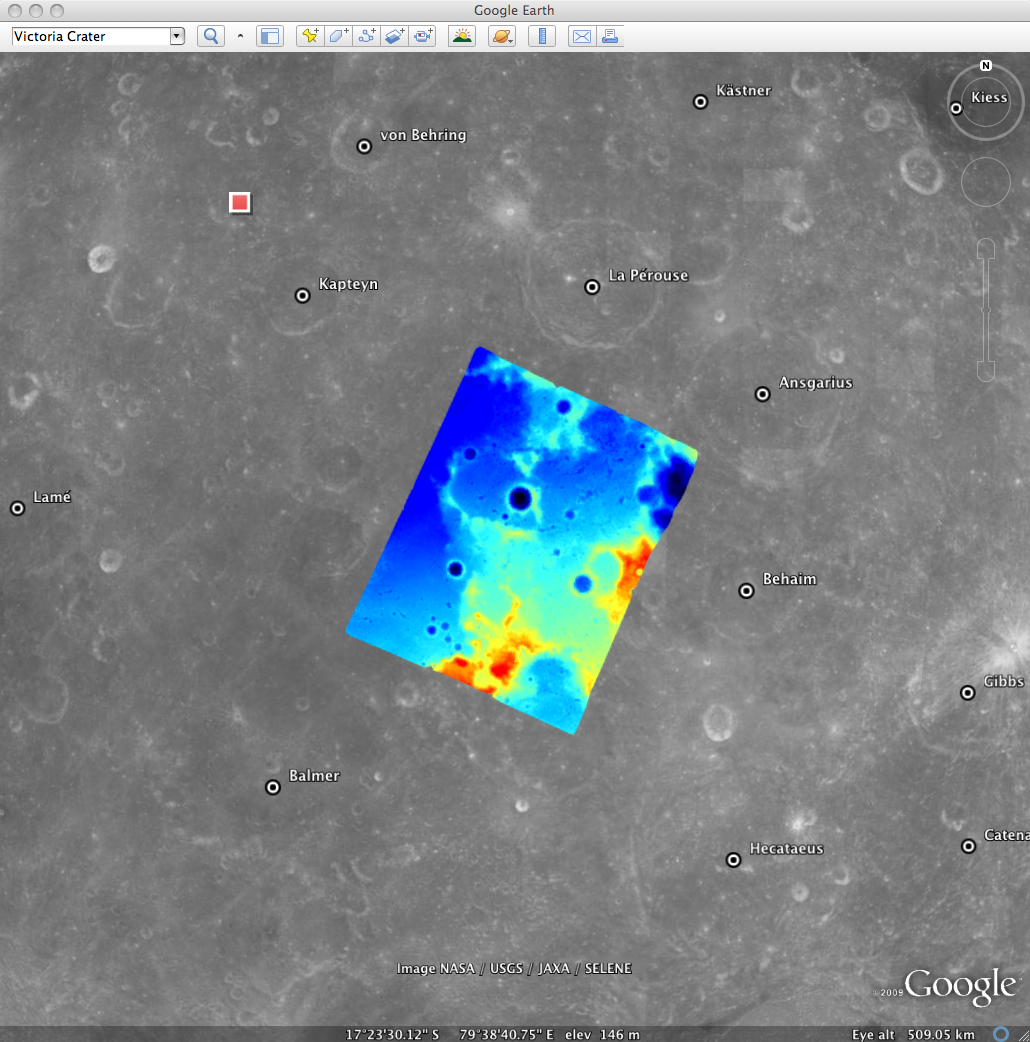
\includegraphics[width=3in]{images/examples/metric/metric_ge_example.png}}
\caption{Example output possible with Apollo Metric frames AS15-M-2380 and AS15-M-2381.}
\label{fig:metric_example}
\end{figure}

\pagebreak

\subsubsection*{Commands}

Process Apollo TIFF files into \ac{ISIS}.
\begin{verbatim}
  ISIS 3> reduce from=AS15-M-2380.cub to=sub4-AS15-M-2380.cub sscale=4 lscale=4
  ISIS 3> reduce from=AS15-M-2381.cub to=sub4-AS15-M-2381.cub sscale=4 lscale=4
  ISIS 3> spiceinit from=sub4-AS15-M-2380.cub
  ISIS 3> spiceinit from=sub4-AS15-M-2381.cub
  ISIS 3> mkdir result
  ISIS 3> stereo sub4-AS15-M-2380.cub sub4-AS15-M-2381.cub result/output
\end{verbatim}

\subsubsection*{stereo.default}

The stereo.default example file works generally well with all Apollo pairs.

%% \pagebreak

%% \section{MESSENGER MDIS}

%% These results are a proof of concept showing off the strength of
%% building the Stereo Pipeline on top of \ac{ISIS}. Support for processing
%% MDIS stereo pairs was not a goal during our design of the software,
%% but the fact that an MDIS camera model exists in ISIS means that
%% it too can be processed by the Stereo Pipeline.

%% For future mappers, we suggest checking out Mercury Flyby 3 data which
%% was not available at the time of this writing. Flyby 3 and Flyby 2
%% seem to have covered some of the same terrain with the narrow angle
%% camera.

%% \subsection{Wide Angle on flyby 2}

%% In most flyby imagery it is very hard to find good stereo pairs.
%% This pair was taken from a single flyby just seconds apart. Note
%% also that this pair is taken from different wavelengths (the letter
%% at the end of the filename designates the current filter being used
%% on the wide angle camera). Unfortunately there is not enough of a
%% perspective change here to make anything other than the spherical
%% surface, but that alone is still an interesting result nonetheless.

%% \begin{figure}[h!]
%% \begin{minipage}{4in}
%% 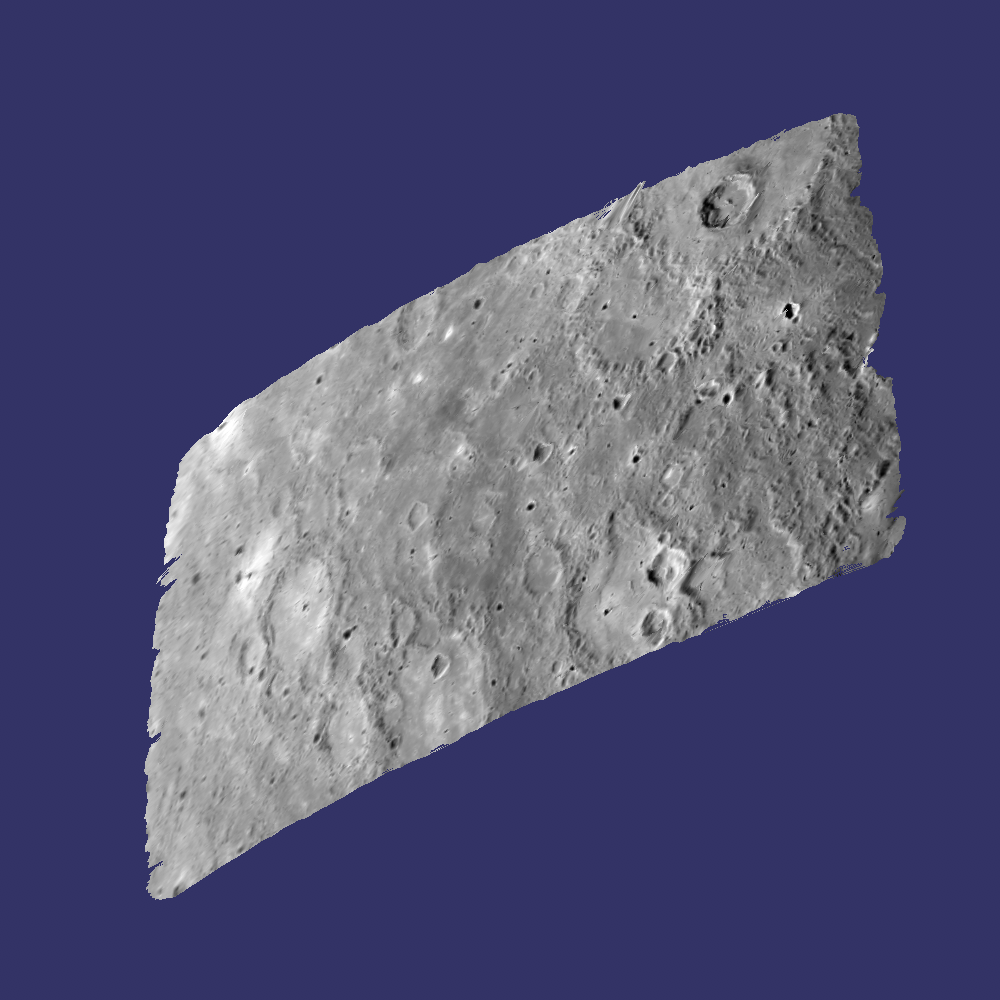
\includegraphics[width=4in]{images/examples/mdis/mdis_wide_example.png}
%% \end{minipage}
%% \hfill
%% \begin{minipage}{2in}
%%   \caption{ A rough attempt at stereo reconstruction from MDIS imagery. }
%%   \label{fig:mdis_attempt}
%% \end{minipage}
%% \end{figure}

%% \subsubsection*{Commands}

%% \begin{verbatim}
%%   ISIS 3> mdis2isis from=EW0108825359A.IMG to=EW0108825359A.cub
%%   ISIS 3> mdis2isis from=EW0108825379C.IMG to=EW0108825379C.cub
%%   ISIS 3> spiceinit from=EW0108825359A.cub
%%   ISIS 3> spiceinit from=EW0108825359C.cub
%%   ISIS 3> mkdir result
%%   ISIS 3> stereo EW0108825359A.cub EW0108825379C.cub stereo/output
%% \end{verbatim}

%% \subsubsection*{stereo.default}

%% \begin{center}\begin{minipage}{5.5in}
%% \begin{Verbatim}[frame=single,fontsize=\small,label=stereo.default for MDIS]
%%     ### PREPROCESSING

%%     DO_INTERESTPOINT_ALIGNMENT 1
%%     INTERESTPOINT_ALIGNMENT_SUBSAMPLING 0
%%     DO_EPIPOLAR_ALIGNMENT 0

%%     FORCE_USE_ENTIRE_RANGE 0
%%     DO_INDIVIDUAL_NORMALIZATION 1

%%     PREPROCESSING_FILTER_MODE 2

%%     SLOG_KERNEL_WIDTH 1.5

%%     ### CORRELATION

%%     COST_BLUR 5
%%     COST_MODE 0

%%     H_KERNEL 25
%%     V_KERNEL 25

%%     H_CORR_MIN -10
%%     H_CORR_MAX 10
%%     V_CORR_MIN -2
%%     V_CORR_MAX 2

%%     SUBPIXEL_MODE 2

%%     SUBPIXEL_H_KERNEL 19
%%     SUBPIXEL_V_KERNEL 19

%%     ### FILTERING

%%     RM_H_HALF_KERN 5
%%     RM_V_HALF_KERN 5
%%     RM_MIN_MATCHES 60 # Units = percent
%%     RM_THRESHOLD 3
%%     RM_CLEANUP_PASSES 1

%%     FILL_HOLES 1

%%     ### DOTCLOUD

%%     NEAR_UNIVERSE_RADIUS 0.0
%%     FAR_UNIVERSE_RADIUS 0.0
%% \end{Verbatim}
%% \end{minipage}\end{center}

\clearpage

\section{Cassini ISS NAC}

This is a proof of concept showing the strength of building the Stereo
Pipeline on top of \ac{ISIS}.  Support for processing ISS NAC stereo pairs
was not a goal during our design of the software, but the fact that a
camera model exists in \ac{ISIS} means that it too can be processed by the
Stereo Pipeline.

Identifying stereo pairs from spacecraft that do not orbit their
target is a challenge. We have found that one usually has to settle
with images that are not ideal: different lighting, little perspective
change, and little or no stereo parallax. So far we have had little
success with Cassini's data, but nonetheless we provide this example
as a potential starting point.

\subsection{Rhea}

Rhea is the second largest moon of Saturn and is roughly a third the
size of our own Moon. This example shows, at the top right of both
images, a giant impact basin named Tirawa that is 220~miles across. The
bright white area south of Tirawa is ejecta from a new crater.  The
lack of texture in this area poses a challenge for our correlator. The
results are just barely useful: the Tirawa impact can barely be made
out in the 3D data while the new crater and ejecta become only noise.

\begin{figure}[p]
\centering
  \subfigure[{\tt Original Left Image}]{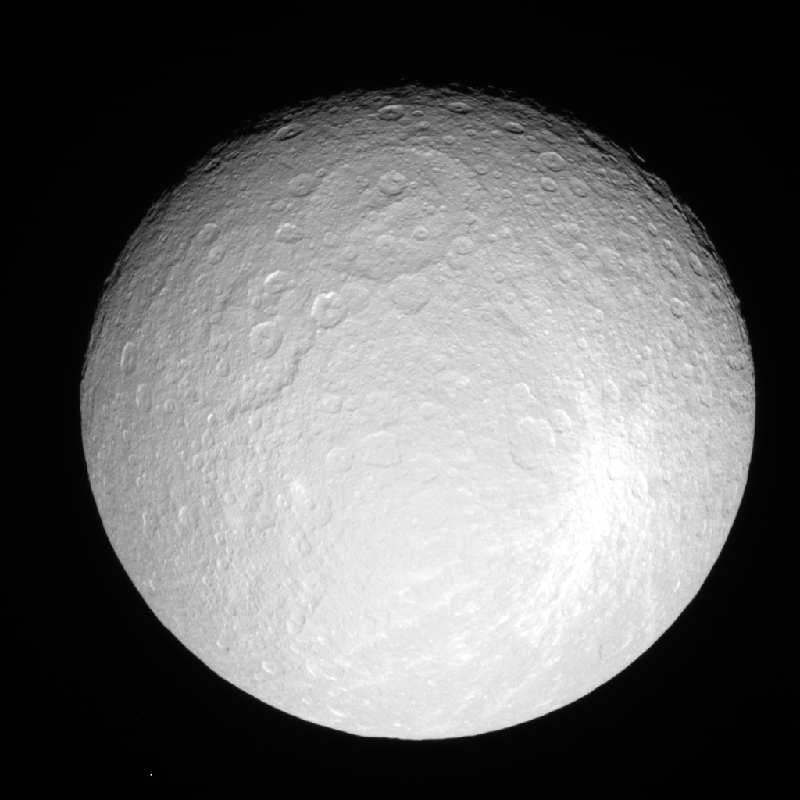
\includegraphics[width=3in]{images/examples/cassini/cassini_rhea_L.png}}
  \hfil
  \subfigure[{\tt Original Right Image}]{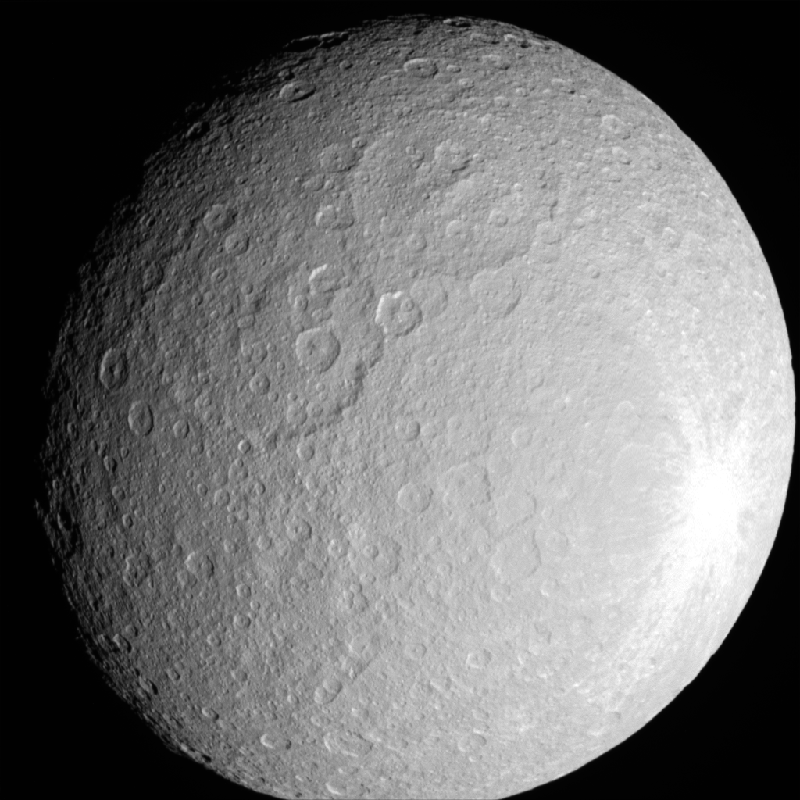
\includegraphics[width=3in]{images/examples/cassini/cassini_rhea_R.png}}
  \\
  \subfigure[{\tt Map Projected Left}]{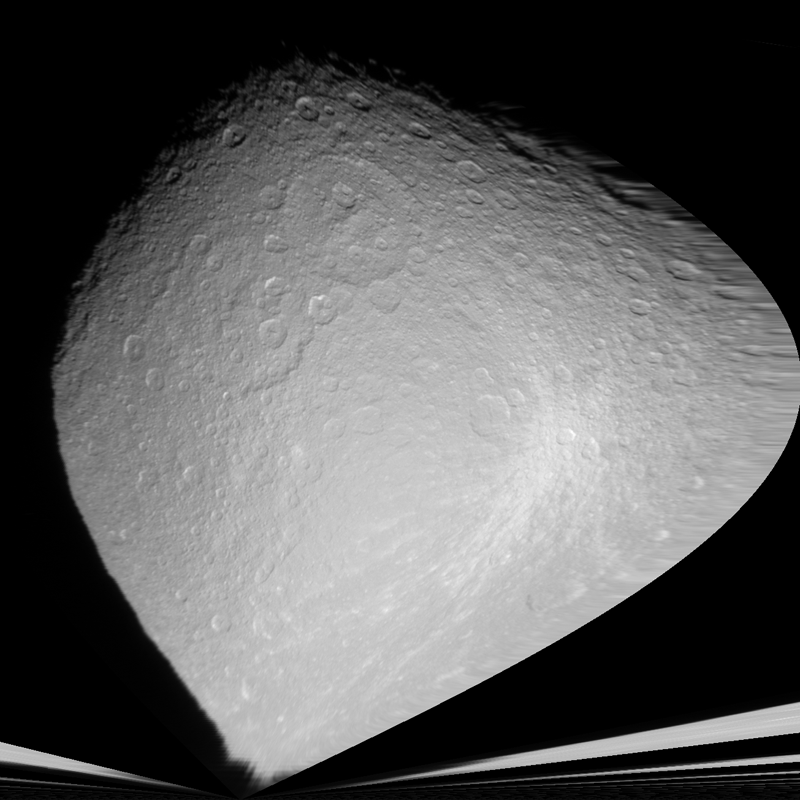
\includegraphics[width=3in]{images/examples/cassini/cassini_rhea_map.png}}
  \hfil
  \subfigure[{\tt 3D Rendering}]{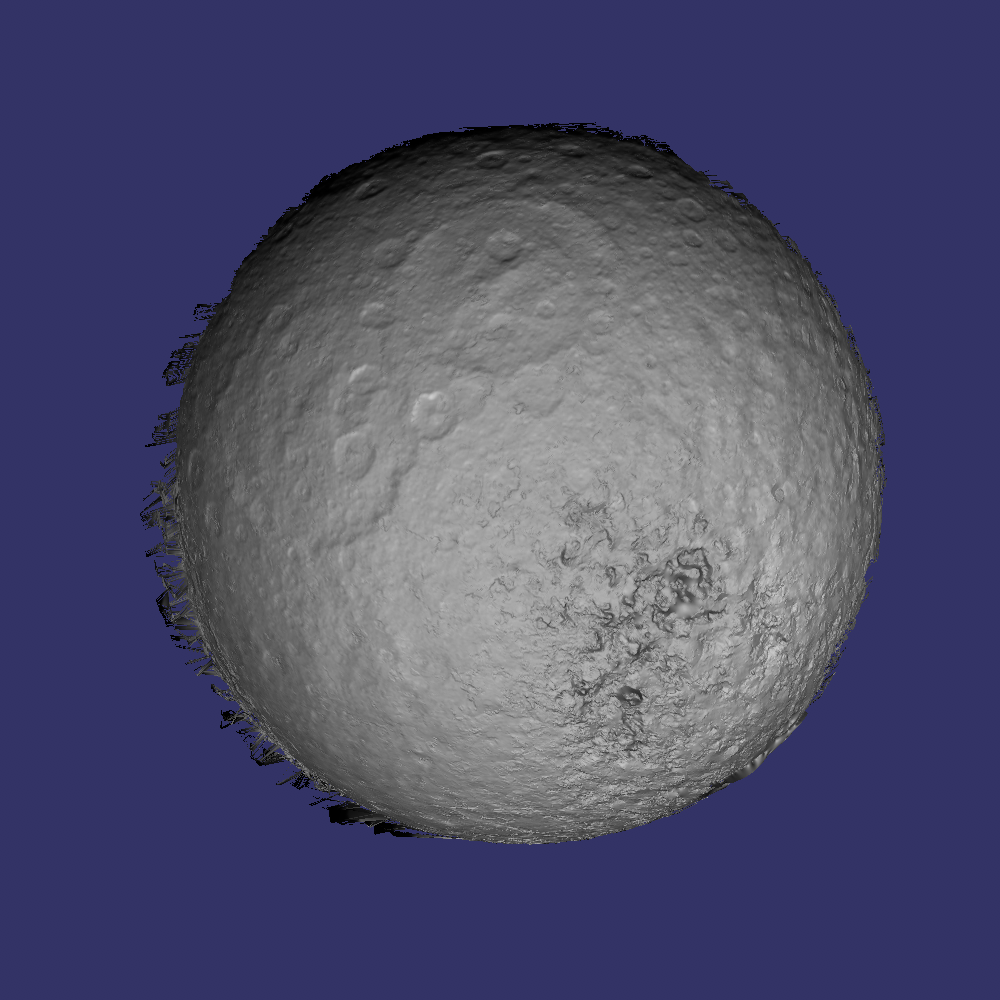
\includegraphics[width=3in]{images/examples/cassini/cassini_rhea.png}}
\caption{Example output of what is possible with Cassini's ISS NAC}
\label{fig:cassini-exampe}
\end{figure}

\subsubsection*{Commands}

Download the N1511700120\_1.IMG and W1567133629\_1.IMG images and their label (.LBL) files from the \ac{PDS}.
\begin{verbatim}
  ISIS 3> ciss2isis f=N1511700120_1.LBL t=N1511700120_1.cub
  ISIS 3> ciss2isis f=W1567133629_1.LBL t=W1567133629_1.cub
  ISIS 3> cisscal from=N1511700120_1.cub to=N1511700120_1.lev1.cub
  ISIS 3> cisscal from=W1567133629_1.cub to=W1567133629_1.lev1.cub
  ISIS 3> fillgap from=W1567133629_1.lev1.cub to=W1567133629_1.fill.cub %Only one image
                                                                        %exhibits the problem
  ISIS 3> cubenorm from=N1511700120_1.lev1.cub to=N1511700120_1.norm.cub
  ISIS 3> cubenorm from=W1567133629_1.fill.cub to=W1567133629_1.norm.cub
  ISIS 3> spiceinit fr= N1511700120_1.norm.cub
  ISIS 3> spiceinit fr= W1567133629_1.norm.cub
  ISIS 3> cam2map from=N1511700120_1.norm.cub to=N1511700120_1.map.cub
  ISIS 3> cam2map from=W1567133629_1.norm.cub map=N1511700120_1.map.cub \
  ISIS 3>           to=W1567133629_1.map.cub matchmap=true
  ISIS 3> ls *.map.cub > fromlist
  ISIS 3> ls N*.map.cub > holdlist
  ISIS 3> equalizer fromlist=fromlist holdlist=holdlist
  ISIS 3> mkdir result
  ISIS 3> stereo N1511700120_1.map.equ.cub W1567133629_1.map.equ.cub result/rhea
\end{verbatim}

\subsubsection*{stereo.default}

\begin{center}\begin{minipage}{5.5in}
\begin{Verbatim}[frame=single,fontsize=\small,label=stereo.default for Cassini ISS]
    ### PREPROCESSING
    alignment-method None
    force-use-entire-range
    individually-normalize

    ### CORRELATION
    prefilter-mode 2
    prefilter-kernel-width 1.5

    cost-mode 2

    corr-kernel 25 25
    corr-search -55 -2 -5 10

    subpixel-mode 3
    subpixel-kernel 21 21

    ### FILTERING
    rm-half-kernel 5 5
    rm-min-matches 60 # Units = percent
    rm-threshold 3
    rm-cleanup-passes 1

\end{Verbatim}
\end{minipage}\end{center}
